\documentclass[letterpaper]{article}
\usepackage{underscore}
\usepackage[left=2.0cm, right=2.0cm, top=2.0cm]{geometry}
\usepackage[utf8]{inputenc}
\usepackage{graphicx}
\usepackage{graphics}
\usepackage[spanish]{babel}
\usepackage{lipsum}
\usepackage{float}
\usepackage{xcolor}
\usepackage{colortbl}
\usepackage{subfigure}
\usepackage{color}

\title{EV\_2\_1\_Diseño\_del\_puente\_H}
\author{Alcantar Diaz Joel Alejandro \\\&\&\\ Ledesma Hernández Miguel Ángel}

\date{10/24/2019}

\begin{document}

\maketitle
\vspace{2cm}
\begin{center}
    
\includegraphics[scale=0.5]{Img/UPZMGlog.png}
\end{center}
\vspace{2cm}
\begin{large}
\begin{center}
Universidad Politécnica de la zona metropolitana de Guadalajara\\
Sistemas Electrónicos de interfaz\\
4-A Mecatrónica\\
\end{center}
\end{large}
\newpage
\begin{huge}
\textbf{Introducción:}\\\\
\end{huge}
La pracita consta de la creación de un puente H en conjunción con otros sistemas desarrollados anteriormente, con el uso de arduino, relays y botones simulando un PLC y el uso de transistores de potencia para la práctica.\\\\
\vspace{.2cm}
\begin{huge}
\textbf{Objetivos de la práctica:}\\
\end{huge}
Crear puente H en conjunto con practicas pasadas\\


\begin{huge}
\textbf{¿Cómo funciona el puente H?:}\\\\
\end{huge}
El puente H es un dispositivo electrónico creado con base a la conjunción de distintos elementos electrónicos tales como mosfet diodo que en este caso no son necesarios puesto que nuestro modelo de mosfet vienen incluidos resistencias y un motor para la comprobación del funcionamiento del puente H.\\
El funcionamiento de este puente H consta de tres procesos Qué es la captación del botón la emisión del arduino y el proceso del puente H el mosfet al recibir la señal de El arduino en la entrada gate permite el flujo de la corriente qué encenderán a nuestro motor dependiendo de la polaridad de nuestra parte del puente H lo que se hace es la inversión por parte de los dos mosfet los cuales están cruzados.\\
Explicando el funcionamiento de presionar el botón cuando nosotros presionamos el botón permitimos el flujo de la corriente hacia la base lo que permitirá el pasó por el colector al emisor esta configuración es duplicada para poder " cerrar el circuito" y mover el motor ahora se crea un espejo de este es decir un inverso lo cual invertirá el giro del motor.
\\\\
\begin{huge}
\textbf{Tabla de Materiales:}\\
\end{huge}


    \begin{table}[h]
\begin{tabular}{|l|l|}
\hline
{\color[HTML]{3166FF} \textbf{Equipo}} & {\color[HTML]{CB0000} \textbf{Componentes}} \\ \hline
Regulador {[}5, 12, 5{]}V              & Relays                                      \\ \hline
Arduino uno                            & Leds                                        \\ \hline
Multímetro                             & Resistencias{[}Varias{]}                    \\ \hline
Motor                                  & Push button                                 \\ \hline
Computadora                            & Cables                                      \\ \hline
                                       & 2n2222A                                     \\ \hline
                                       & IRF640N                                     \\ \hline
\end{tabular}
\end{table}

\begin{huge}
\textbf{Desarrollo:}\\
\end{huge}
Se separó la práctica en cuatro módulos para facilitar la comprensión del sistema y su analisis en caso de fallas, uno de estos es el módulo de botones; en este módulo colocamos los botones en la protoboard de manera que se puedan conectar posteriormente al arduino uno y de esta manera poder programar la pulsación de cada uno de los botones, así cuando uno de estos esté en estado HIGH, emita un pulso que encienda un led y el relevador, que este ya es parte de la tercera sección. La segunda sección es la programación y conección del arduino, usandolo como una especie de PLC que comunica las entradas de los botones con las salidas de los relevadores. De la conección de los relevadores nos manda a la cuarta sección que es la parte del puente H, que es la parte principal.
\\
Para hacer el puente H se toman los 4 mosfet "IRF640N" y se conectan con base a la siguiente imagen[datasheet]:\\
\begin{figure}[htbp]
    \centering
    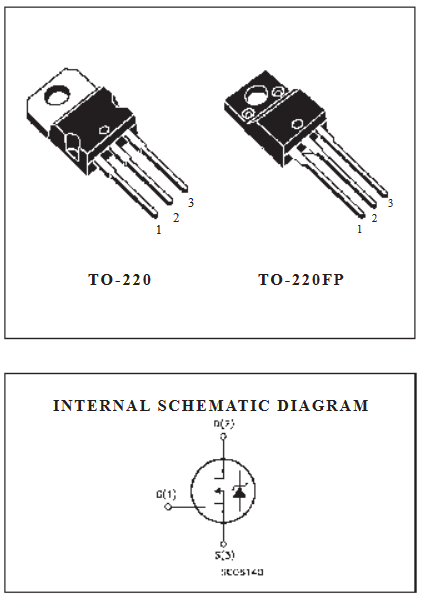
\includegraphics[width=5cm]{Img/datasheetIRF.PNG}
    \caption{Datasheet IRF640N}
    \label{fig:my_lab4el}
\end{figure}\\
Una vez visto el datasheet lo conectamos en una forma de H o doble L para poder organizar facilmente las conecciones basandonos en el datasheet.\\
\newpage
\begin{figure}[htbp]
    \centering
    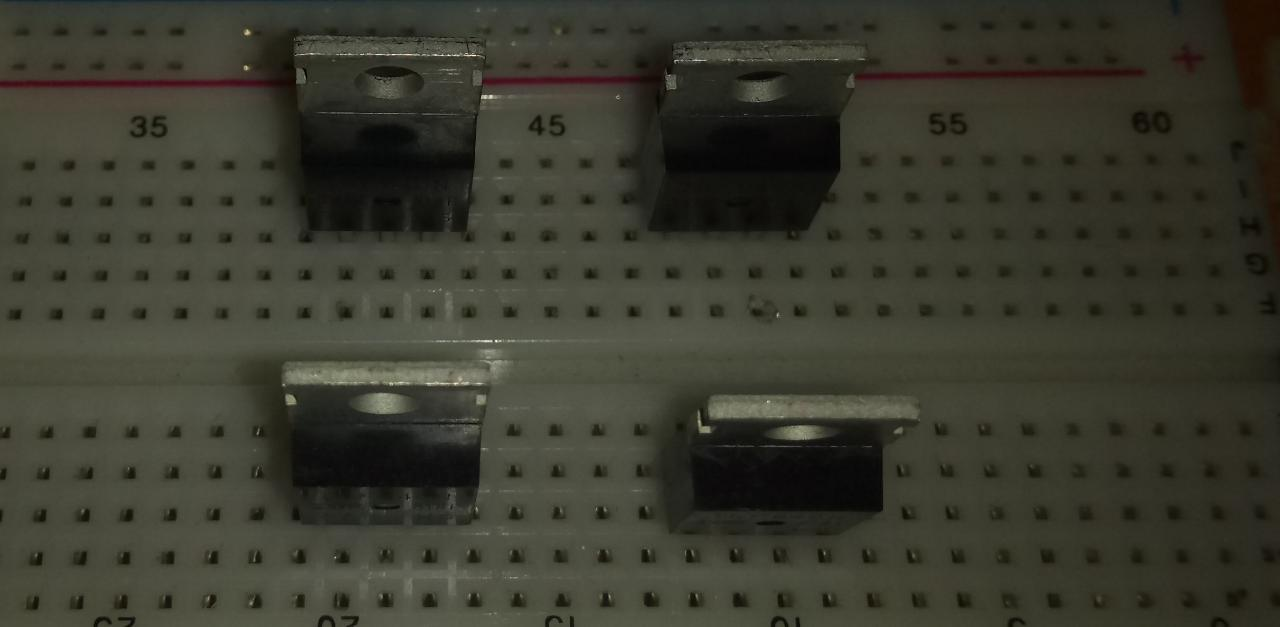
\includegraphics[width=15cm]{Img/puenteH1.jpeg}
    \caption{Forma de H}
    \label{fig:my_l3abel}
\end{figure}
Se ponen despues resistencias en la segunda patita y estas en siguientes pasos será conectado a los botones.\\
\newpage
\begin{figure}[htbp]
    \centering
    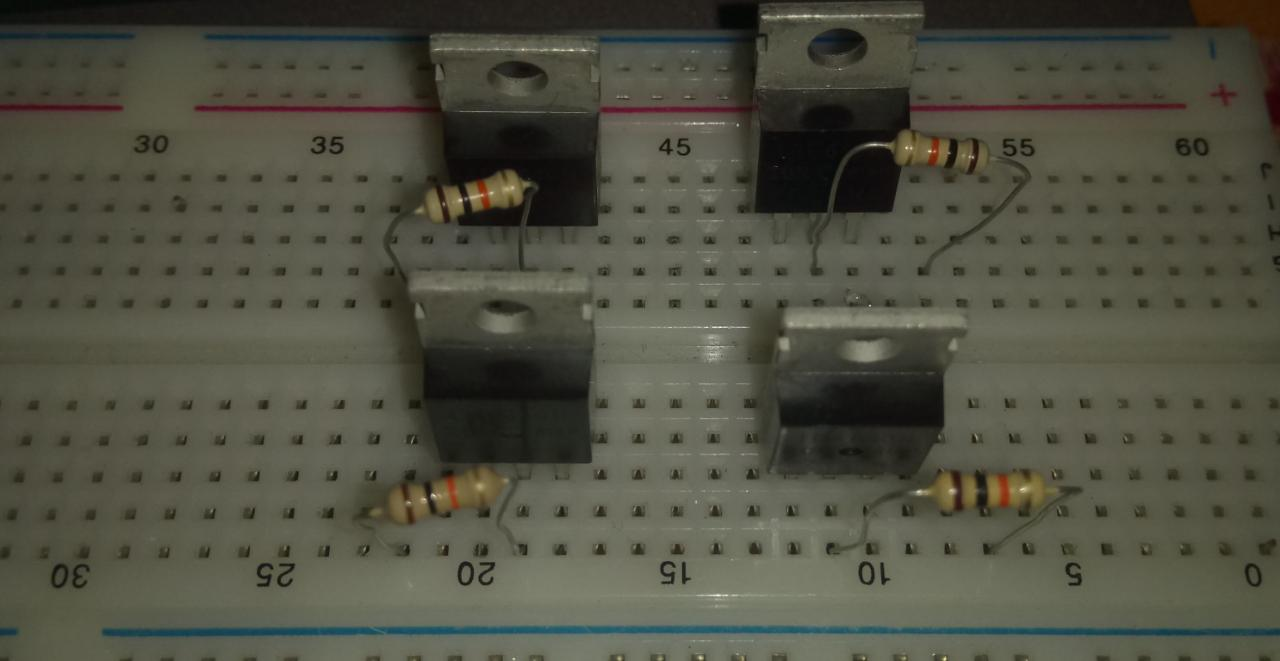
\includegraphics[width=15cm]{Img/puenteH2.jpeg}
    \caption{Resistencias}
    \label{fig:my_lab2el}
\end{figure}
\newpage
Se conectan las patas del contrario creando un cruce para posteriormente conectar las resistencias y las patitas sobrantes al negativo de el cuadrante inferior como se ven en las siguientes imagenes.\\
\begin{figure}[htbp]
    \centering
    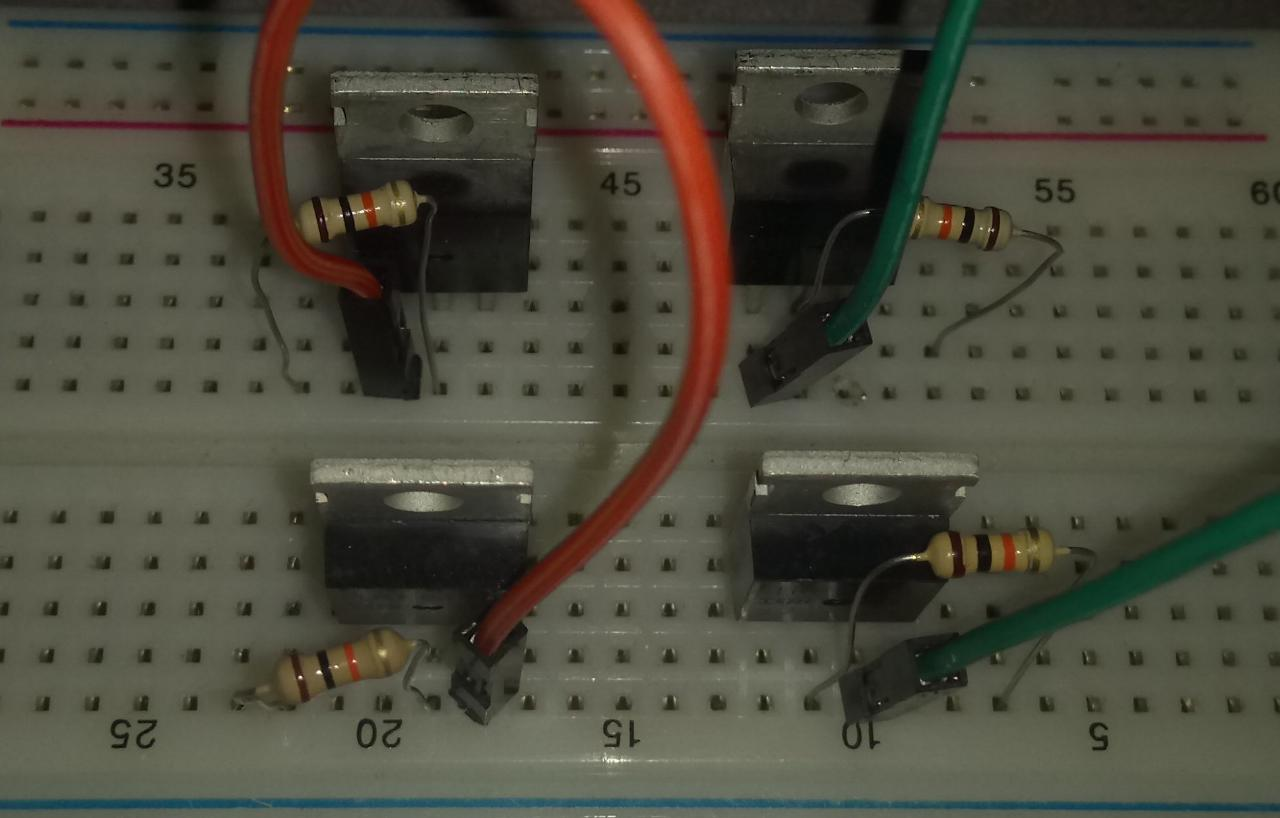
\includegraphics[width=15cm]{Img/puenteH3.jpeg}
    \caption{cruce de mosfet}
    \label{fig:my_labe1l}
\end{figure}
Esta parte nos muestra como de la patita numero uno conectamos en la patita numero dos para crear el puente H utilizando como base la datasheet que se nos proporciona con el componente\\

\begin{figure}[htbp]
    \centering
    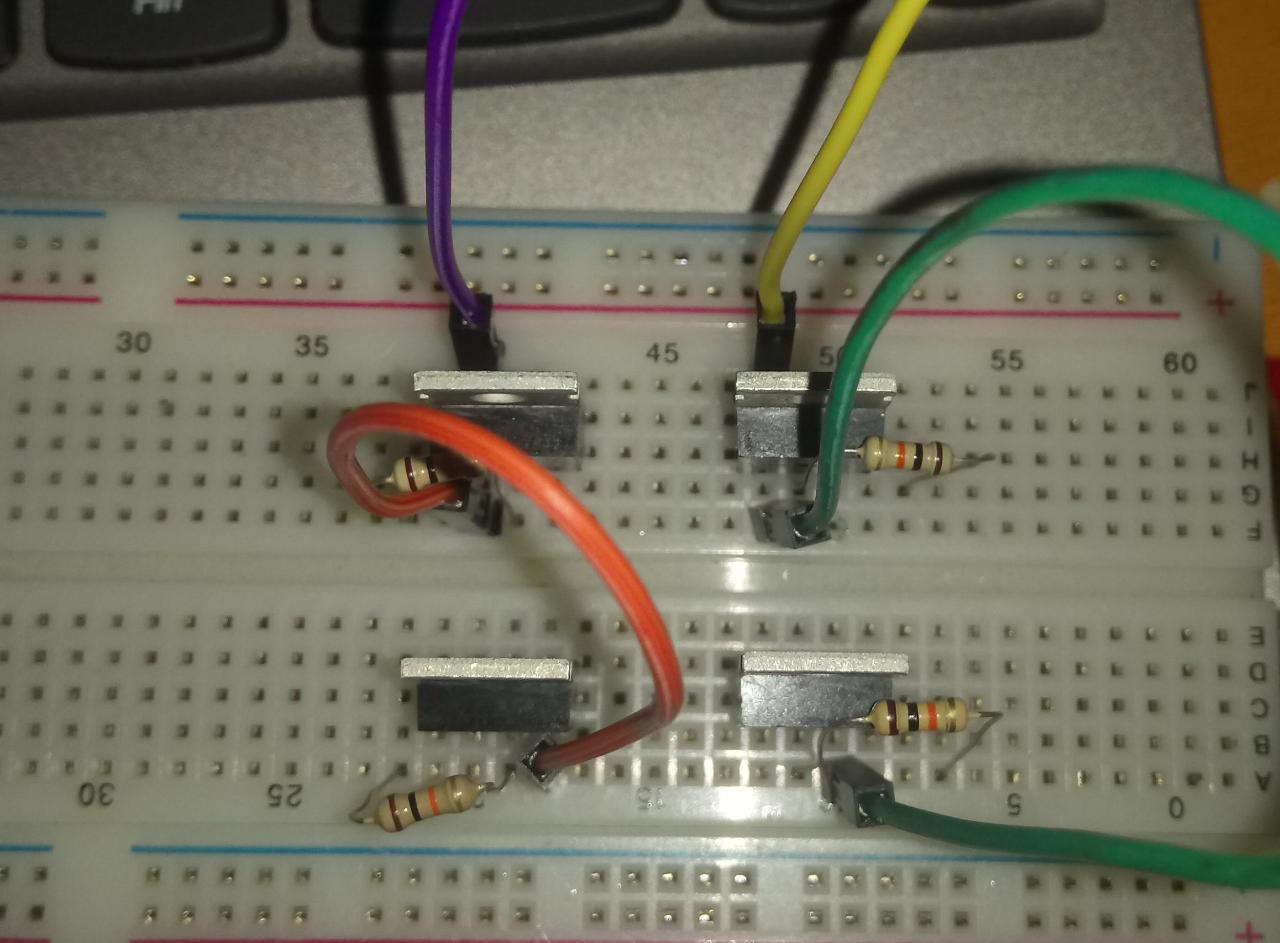
\includegraphics[width=8cm]{Img/puenteH4.jpeg}
    \caption{salidas del motor y botones}
    \label{fig:my_label}
\end{figure}
\begin{figure}[htbp]
    \centering
    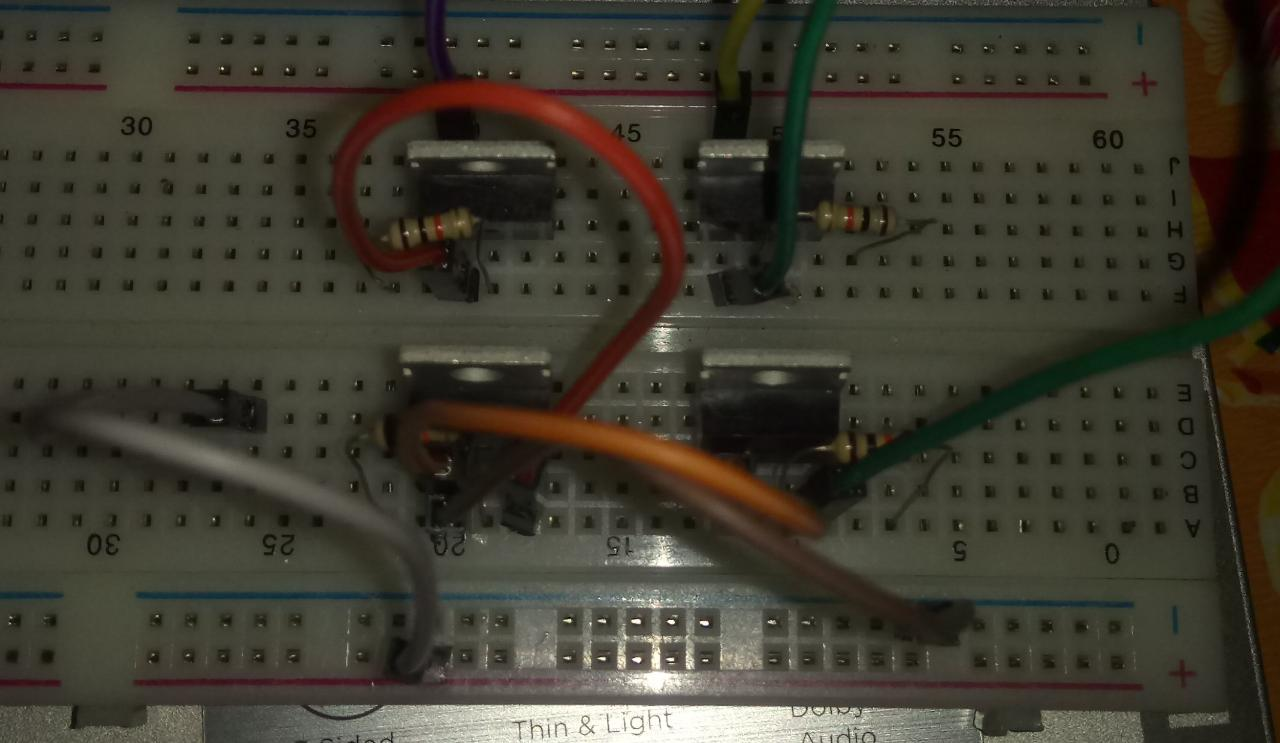
\includegraphics[width=15cm]{Img/puenteH5.jpeg}
    \caption{polaridades}
    \label{fig:my_label1}
\end{figure}
\newpage
\textbf{Conclusiones}\\
\begin{large}
    De esta practica se puede concluir la funcionalidad que tiene un transistor o mosfet frente a un switch ya que su actuacion es mas rapida y su desgaste es menor que el de un actuador mecanico como lo es un relay a parte de que el consumo de estos es mucho mayor al de un mosfet ya que un mosfet puede actuar de interruptor con una corriente muy pequeña, en algunos casos de 10mA en comparacion a los 400mA que consume un relay de 12v.\\
\end{large}
\begin{thebibliography}{}
\bibitem{queso} \textit{Como conectar un MOSFET de potencia a un microcontrolador.} Recuperado el 23/10/2019 de:\\ https://www.inventable.eu/como-conectar-un-mosfet-a-un-microcontrolador/

\end{thebibliography}
\end{document}
